\subsubsection{2.3. Kết quả kiểm thử trên mô hình CNN + MGAT + FastKAN/MLP với toàn bộ phương thức}
\indent\indent Dưới đây là kết quả kiểm thử chi tiết của 12 mô hình CNN backbone + MGAT + FastKAN/MLP với toàn bộ phương thức, trong đó các giá trị được lấy từ lần chạy đạt kết quả cao nhất.\vspace{0.3cm}

%===================================================================
\textbf{* ResNet18 + MGAT + FastKAN/MLP:} 
\begin{table}[H] 
\centering 
\renewcommand{\arraystretch}{1.08} 
\caption{\centering Classification report của FastKAN(1) và MLP(2) trên toàn bộ phương thức với backbone ResNet18} 
\begin{tabular}{lccccccc} 
\hline \textbf{Lớp} & \textbf{P(1)} & \textbf{R(1)} & \textbf{F1(1)} & \textbf{P(2)} & \textbf{R(2)} & \textbf{F1(2)} & \textbf{Support} \\ \hline

cho-noi-cai-rang 
& 1.0000 & 0.9556 & \textbf{0.9773} 
& 0.9333 & 0.9333 & 0.9333 & 45 \\

dua-bo-bay-nui 
& 1.0000 & 1.0000 & \textbf{1.0000} 
& 0.9574 & 1.0000 & 0.9783 & 45 \\

hoi-lim 
& 0.9762 & 0.9111 & \textbf{0.9425} 
& 0.9130 & 0.9333 & 0.9231 & 45 \\

le-hoi-nghinh-ong 
& 0.9000 & 0.8000 & \textbf{0.8471} 
& 0.8261 & 0.8444 & 0.8352 & 45 \\

nghe-dan-tre 
& 1.0000 & 1.0000 & \textbf{1.0000} 
& 0.9565 & 0.9778 & 0.9670 & 45 \\

nghe-det-chieu 
& 0.9574 & 1.0000 & \textbf{0.9783} 
& 0.9348 & 0.9556 & 0.9451 & 45 \\

ok-om-bok 
& 0.9574 & 1.0000 & \textbf{0.9783} 
& 1.0000 & 0.8444 & 0.9157 & 45 \\

via-ba-chua-xu-nui-sam 
& 0.8235 & 0.9333 & \textbf{0.8750} 
& 0.8478 & 0.8667 & 0.8571 & 45 \\ 
\hline

\textbf{Accuracy} 
& & & \textbf{0.9500} 
& & & 0.9194 & 360 \\

\textbf{Macro avg} 
& \textbf{0.9518} & \textbf{0.9500} & \textbf{0.9498} 
& 0.9211 & 0.9194 & 0.9193 & 360 \\

\textbf{Weighted avg} 
& \textbf{0.9518} & \textbf{0.9500} & \textbf{0.9498} 
& 0.9211 & 0.9194 & 0.9193 & 360 \\ 
\hline 
\end{tabular} 
\end{table}

%===================================================================
\textbf{* RegNetX400MF + MGAT + FastKAN/MLP:}
\begin{table}[H]
\centering
\renewcommand{\arraystretch}{1.08}
\caption{\centering Classification report của FastKAN(1) và MLP(2) trên toàn bộ phương thức với backbone RegNetX400MF}
\begin{tabular}{lccccccc}
\hline
\textbf{Lớp} &
\textbf{P(1)} & \textbf{R(1)} & \textbf{F1(1)} &
\textbf{P(2)} & \textbf{R(2)} & \textbf{F1(2)} &
\textbf{Support} \\
\hline

cho-noi-cai-rang
& 0.9778 & 0.9778 & \textbf{0.9778}
& 0.9565 & 0.9778 & 0.9670 & 45 \\

dua-bo-bay-nui
& 1.0000 & 1.0000 & \textbf{1.0000}
& 0.9375 & 1.0000 & 0.9677 & 45 \\

hoi-lim
& 0.8889 & 0.8889 & 0.8889
& 0.9318 & 0.9111 & \textbf{0.9213} & 45 \\

le-hoi-nghinh-ong
& 0.7727 & 0.7556 & 0.7640
& 0.8649 & 0.7111 & \textbf{0.7805} & 45 \\

nghe-dan-tre
& 1.0000 & 1.0000 & \textbf{1.0000}
& 0.9783 & 1.0000 & 0.9890 & 45 \\

nghe-det-chieu
& 0.9778 & 0.9778 & \textbf{0.9778}
& 1.0000 & 0.8889 & 0.9412 & 45 \\

ok-om-bok
& 0.9545 & 0.9333 & 0.9438
& 0.9556 & 0.9556 & \textbf{0.9556} & 45 \\

via-ba-chua-xu-nui-sam
& 0.7660 & 0.8000 & 0.7826
& 0.7593 & 0.9111 & \textbf{0.8283} & 45 \\
\hline

\textbf{Accuracy}
& & & 0.9167
& & & \textbf{0.9194} & 360 \\

\textbf{Macro avg}
& 0.9172 & 0.9167 & 0.9169
& \textbf{0.9230} & \textbf{0.9194} & \textbf{0.9188} & 360 \\

\textbf{Weighted avg}
& 0.9172 & 0.9167 & 0.9169
& \textbf{0.9230} & \textbf{0.9194} & \textbf{0.9188} & 360 \\
\hline
\end{tabular}
\end{table}
%===================================================================
\textbf{* MobileNetV3 Large + MGAT + FastKAN/MLP:}
\begin{table}[H]
\centering
\renewcommand{\arraystretch}{1.08}
\caption{\centering Classification report của FastKAN(1) và MLP(2) trên toàn bộ phương thức với backbone MobileNetV3 Large}
\label{tab:CRMobileNetV3LargeMGATFastKANMLP}
\begin{tabular}{lccccccc}
\hline
\textbf{Lớp} &
\textbf{P(1)} & \textbf{R(1)} & \textbf{F1(1)} &
\textbf{P(2)} & \textbf{R(2)} & \textbf{F1(2)} &
\textbf{Support} \\
\hline
cho-noi-cai-rang
& 0.9184 & 1.0000 & 0.9574
& 0.9778 & 0.9778 & \textbf{0.9778} & 45 \\

dua-bo-bay-nui
& 1.0000 & 1.0000 & \textbf{1.0000}
& 0.9783 & 1.0000 & 0.9890 & 45 \\

hoi-lim
& 0.9111 & 0.9111 & \textbf{0.9111}
& 0.8333 & 0.8889 & 0.8602 & 45 \\

le-hoi-nghinh-ong
& 0.8780 & 0.8000 & \textbf{0.8372}
& 0.8684 & 0.7333 & 0.7952 & 45 \\

nghe-dan-tre
& 1.0000 & 0.9778 & \textbf{0.9888}
& 0.9778 & 0.9778 & 0.9778 & 45 \\

nghe-det-chieu
& 0.9762 & 0.9111 & 0.9425
& 0.9767 & 0.9333 & \textbf{0.9545} & 45 \\

ok-om-bok
& 0.9773 & 0.9556 & \textbf{0.9663}
& 0.9130 & 0.9333 & 0.9231 & 45 \\

via-ba-chua-xu-nui-sam
& 0.8000 & 0.8889 & \textbf{0.8421}
& 0.7551 & 0.8222 & 0.7872 & 45 \\
\hline

\textbf{Accuracy}
& & & {\textbf{0.9306}}
& & & {0.9083} & 360 \\

\textbf{Macro avg}
& \textbf{0.9326} & \textbf{0.9306} & \textbf{0.9307}
& 0.9101 & 0.9083 & 0.9081 & 360 \\

\textbf{Weighted avg}
& \textbf{0.9326} & \textbf{0.9306} & \textbf{0.9307}
& 0.9101 & 0.9083 & 0.9081 & 360 \\
\hline
\end{tabular}
\end{table}
%===================================================================
\textbf{* MobileNetV3 Small + MGAT + FastKAN/MLP:}
\begin{table}[H]
\centering
\renewcommand{\arraystretch}{1.08}
\caption{\centering Classification report của FastKAN(1) và MLP(2) trên toàn bộ phương thức với backbone MobileNetV3 Small}
\begin{tabular}{lccccccc}
\hline
\textbf{Lớp} &
\textbf{P(1)} & \textbf{R(1)} & \textbf{F1(1)} &
\textbf{P(2)} & \textbf{R(2)} & \textbf{F1(2)} &
\textbf{Support} \\
\hline

cho-noi-cai-rang
& 0.9778 & 0.9778 & \textbf{0.9778}
& 0.8980 & 0.9778 & 0.9362 & 45 \\

dua-bo-bay-nui
& 1.0000 & 0.9778 & 0.9888
& 1.0000 & 1.0000 & \textbf{1.0000} & 45 \\

hoi-lim
& 0.9302 & 0.8889 & 0.9091
& 0.9111 & 0.9111 & \textbf{0.9111} & 45 \\

le-hoi-nghinh-ong
& 0.7857 & 0.7333 & 0.7586
& 0.8372 & 0.8000 & \textbf{0.8182} & 45 \\

nghe-dan-tre
& 0.9773 & 0.9556 & 0.9663
& 1.0000 & 0.9778 & \textbf{0.9888} & 45 \\

nghe-det-chieu
& 0.9130 & 0.9333 & 0.9231
& 0.9535 & 0.9111 & \textbf{0.9318} & 45 \\

ok-om-bok
& 0.9565 & 0.9778 & \textbf{0.9670}
& 0.9556 & 0.9556 & 0.9556 & 45 \\

via-ba-chua-xu-nui-sam
& 0.7600 & 0.8444 & 0.8000
& 0.8261 & 0.8444 & \textbf{0.8352} & 45 \\
\hline

\textbf{Accuracy}
& & & 0.9111
& & & \textbf{0.9222} & 360 \\

\textbf{Macro avg}
& 0.9126 & 0.9111 & 0.9113
& \textbf{0.9227} & \textbf{0.9222} & \textbf{0.9221} & 360 \\

\textbf{Weighted avg}
& 0.9126 & 0.9111 & 0.9113
& \textbf{0.9227} & \textbf{0.9222} & \textbf{0.9221} & 360 \\
\hline
\end{tabular}
\end{table}
%===================================================================
\textbf{* DenseNet121 + MGAT + FastKAN/MLP:}
\begin{table}[H]
\centering
\renewcommand{\arraystretch}{1.08}
\caption{\centering Classification report của FastKAN(1) và MLP(2) trên toàn bộ phương thức với backbone DenseNet121}
\begin{tabular}{lccccccc}
\hline
\textbf{Lớp} &
\textbf{P(1)} & \textbf{R(1)} & \textbf{F1(1)} &
\textbf{P(2)} & \textbf{R(2)} & \textbf{F1(2)} &
\textbf{Support} \\
\hline

cho-noi-cai-rang
& 1.0000 & 1.0000 & \textbf{1.0000}
& 0.9565 & 0.9778 & 0.9670 & 45 \\

dua-bo-bay-nui
& 1.0000 & 1.0000 & \textbf{1.0000}
& 1.0000 & 1.0000 & \textbf{1.0000} & 45 \\

hoi-lim
& 0.9302 & 0.8889 & 0.9091
& 0.9149 & 0.9556 & \textbf{0.9348} & 45 \\

le-hoi-nghinh-ong
& 0.8750 & 0.9333 & 0.9032
& 0.9111 & 0.9111 & \textbf{0.9111} & 45 \\

nghe-dan-tre
& 1.0000 & 0.9778 & 0.9888
& 0.9783 & 1.0000 & \textbf{0.9890} & 45 \\

nghe-det-chieu
& 0.9783 & 1.0000 & \textbf{0.9890}
& 1.0000 & 0.9556 & 0.9773 & 45 \\

ok-om-bok
& 0.9318 & 0.9111 & 0.9213
& 0.9333 & 0.9333 & \textbf{0.9333} & 45 \\

via-ba-chua-xu-nui-sam
& 0.9333 & 0.9333 & \textbf{0.9333}
& 0.9302 & 0.8889 & 0.9091 & 45 \\
\hline

\textbf{Accuracy}
& & & \textbf{0.9556}
& & & 0.9528 & 360 \\

\textbf{Macro avg}
& \textbf{0.9561} & \textbf{0.9556} & \textbf{0.9556}
& 0.9530 & 0.9528 & 0.9527 & 360 \\

\textbf{Weighted avg}
& \textbf{0.9561} & \textbf{0.9556} & \textbf{0.9556}
& 0.9530 & 0.9528 & 0.9527 & 360 \\
\hline
\end{tabular}
\end{table}

%===================================================================
\textbf{* ShuffleNetV2 1.0x + MGAT + FastKAN/MLP:}
\begin{table}[H]
\centering
\renewcommand{\arraystretch}{1.08}
\caption{\centering Classification report của FastKAN(1) và MLP(2) trên toàn bộ phương thức với backbone ShuffleNetV2 1.0x}
\begin{tabular}{lccccccc}
\hline
\textbf{Lớp} &
\textbf{P(1)} & \textbf{R(1)} & \textbf{F1(1)} &
\textbf{P(2)} & \textbf{R(2)} & \textbf{F1(2)} &
\textbf{Support} \\
\hline

cho-noi-cai-rang
& 1.0000 & 0.9111 & \textbf{0.9535}
& 0.9556 & 0.9556 & 0.9556 & 45 \\

dua-bo-bay-nui
& 0.9778 & 0.9778 & 0.9778
& 1.0000 & 0.9778 & \textbf{0.9888} & 45 \\

hoi-lim
& 0.8478 & 0.8667 & 0.8571
& 0.8958 & 0.9556 & \textbf{0.9247} & 45 \\

le-hoi-nghinh-ong
& 0.8333 & 0.8889 & \textbf{0.8602}
& 0.8750 & 0.7778 & 0.8235 & 45 \\

nghe-dan-tre
& 1.0000 & 0.9333 & 0.9655
& 0.9556 & 0.9556 & \textbf{0.9556} & 45 \\

nghe-det-chieu
& 0.8800 & 0.9778 & 0.9263
& 0.9565 & 0.9778 & \textbf{0.9670} & 45 \\

ok-om-bok
& 0.8667 & 0.8667 & 0.8667
& 1.0000 & 0.9333 & \textbf{0.9655} & 45 \\

via-ba-chua-xu-nui-sam
& 0.8837 & 0.8444 & \textbf{0.8636}
& 0.8200 & 0.9111 & 0.8632 & 45 \\
\hline

\textbf{Accuracy}
& & & 0.9083
& & & \textbf{0.9306} & 360 \\

\textbf{Macro avg}
& 0.9112 & 0.9083 & 0.9088
& \textbf{0.9323} & \textbf{0.9306} & \textbf{0.9305} & 360 \\

\textbf{Weighted avg}
& 0.9112 & 0.9083 & 0.9088
& \textbf{0.9323} & \textbf{0.9306} & \textbf{0.9305} & 360 \\
\hline
\end{tabular}
\end{table}

\indent Dựa trên kết quả kiểm thử chi tiết của các mô hình CNN backbone kết hợp với MGAT và FastKAN/MLP trên tập dữ liệu kiểm thử với đầy đủ ba phương thức, có thể rút ra một số nhận xét chính như sau:\vspace{-0.1cm}
\begin{itemize}[label={--}, itemsep=1pt]
    \item Hiệu quả của tiếp cận đa phương thức: So với các mô hình CNN baseline chỉ sử dụng thông tin hình ảnh (với Accuracy trung bình xấp xỉ 0.9-0.91), việc tích hợp thêm dữ liệu văn bản và âm thanh thông qua kiến trúc MGAT giúp cải thiện kết quả một cách đáng kể trên hầu hết các backbone. Mức cải thiện này thể hiện rõ nhất ở các lớp có mức độ nhập nhằng cao trong dữ liệu hình ảnh (\textit{le-hoi-nghinh-ong} và \textit{via-ba-chua-xu-nui-sam}), cho thấy vai trò bổ trợ quan trọng của thông tin ngữ nghĩa và âm thanh trong quá trình phân loại.
    
    \item So sánh FastKAN và MLP trên từng backbone:\vspace{-0.1cm}
    \begin{itemize}[label={+}, itemsep=1pt]
        \item ResNet18: FastKAN thể hiện ưu thế rõ rệt so với MLP. Mô hình ResNet18 kết hợp FastKAN đạt độ chính xác 0.95, cao hơn đáng kể so với 0.9194 của MLP. Đặc biệt, tại lớp khó \textit{via-ba-chua-xu-nui-sam}, FastKAN giúp cải thiện Recall từ 0.87 lên 0.93, cho thấy khả năng mô hình hóa các biên quyết định phi tuyến phức tạp hiệu quả hơn so với cấu trúc MLP truyền thống.
        \item DenseNet121: Đây là backbone cho kết quả cao nhất trong toàn bộ các kết quả kiểm thử, với độ chính xác vượt ngưỡng 0.95 ở cả hai bộ phân lớp FastKAN và MLP. So với mô hình CNN baseline đơn phương thức, mức cải thiện đạt được vào khoảng 5\%, cho thấy sự kết hợp giữa biểu diễn đặc trưng mạnh và tích hợp đa phương thức mang lại hiệu quả đáng kể.
        \item MobileNetV3 Large: FastKAN tiếp tục cho thấy lợi thế với Accuracy đạt 0.9306, so với 0.9083 của MLP. Mô hình đạt kết quả gần như tuyệt đối ở lớp \textit{dua-bo-bay-nui}, đồng thời cải thiện đáng kể F1-Score của lớp \textit{le-hoi-nghinh-ong} (0.8372 so với 0.7952). Điều này cho thấy sự kết hợp giữa một backbone gọn nhẹ và một bộ phân lớp có năng lực biểu diễn cao là một hướng tiếp cận tiềm năng.
        \item Các backbone MobileNetV3 Small, ShuffleNetV2 và RegNet: Trong nhóm các kiến trúc gọn nhẹ hơn, MLP cho kết quả tương đương hoặc nhỉnh hơn FastKAN. Chẳng hạn, với ShuffleNetV2 1.0x, MLP đạt độ chính xác 0.9306 trong khi FastKAN đạt 0.9083. Khi đặc trưng đầu vào từ backbone bị nén mạnh và chứa ít thông tin hơn, độ phức tạp cao của FastKAN có thể dẫn đến hiện tượng overfitting nhẹ, trong khi cấu trúc đơn giản của MLP giúp mô hình duy trì khả năng tổng quát hóa tốt hơn.
    \end{itemize}
\end{itemize}

%===================================================================
Dưới đây là bảng tổng hợp và biểu đồ thể hiện kết quả trung bình của tất cả 12 mô hình CNN backbone + MGAT + FastKAN/MLP:
\begin{table}[H]
\centering
\renewcommand{\arraystretch}{1.2}
\setlength{\tabcolsep}{6pt}
\caption{\centering Kết quả kiểm thử trung bình của tất cả các mô hình CNN backbone + MGAT + FastKAN/MLP trên toàn bộ phương thức}
\begin{tabular}{llcccc}
\hline
\textbf{Backbone Model (+ MGAT)} & \textbf{Classifier} & \textbf{Accuracy} & \textbf{Precision} & \textbf{Recall} & \textbf{F1-Score} \\ 
\hline

% ResNet18
\multirow{2}{*}{ResNet18} 
& FastKAN & \textbf{0.9343} & \textbf{0.9358} & \textbf{0.9343} & \textbf{0.9341} \\
& MLP & 0.9000 & 0.9030 & 0.9000 & 0.8996 \\ 
\hline

% RegNetX400MF
\multirow{2}{*}{RegNetX400MF} 
& FastKAN & 0.9074 & 0.9094 & 0.9074 & 0.9071 \\
& MLP & \textbf{0.9092} & \textbf{0.9134} & \textbf{0.9092} & \textbf{0.9090} \\ 
\hline

% MobileNetV3 Large
\multirow{2}{*}{MobileNetV3 Large} 
& FastKAN & \textbf{0.9260} & \textbf{0.9283} & \textbf{0.9260} & \textbf{0.9258} \\
& MLP & 0.9056 & 0.9059 & 0.9056 & 0.9043 \\ 
\hline

% MobileNetV3 Small
\multirow{2}{*}{MobileNetV3 Small} 
& FastKAN & 0.9055 & 0.9111 & 0.9055 & 0.9041 \\
& MLP & \textbf{0.9120} & \textbf{0.9174} & \textbf{0.9120} & \textbf{0.9118} \\ 
\hline

% DenseNet121
\multirow{2}{*}{DenseNet121} 
& FastKAN & \textbf{0.9435} & \textbf{0.9477} & \textbf{0.9435} & \textbf{0.9438} \\
& MLP & 0.9417 & 0.9455 & 0.9417 & 0.9413 \\ 
\hline

% ShuffleNetV2
\multirow{2}{*}{ShuffleNetV2 1.0x} 
& FastKAN & 0.8981 & 0.9007 & 0.8981 & 0.8980 \\
& MLP & \textbf{0.9204} & \textbf{0.9236} & \textbf{0.9204} & \textbf{0.9203} \\ 
\hline

\end{tabular}
\label{tab:avg_performance_comparison}
\end{table}

\begin{figure}[H]
    \centering
    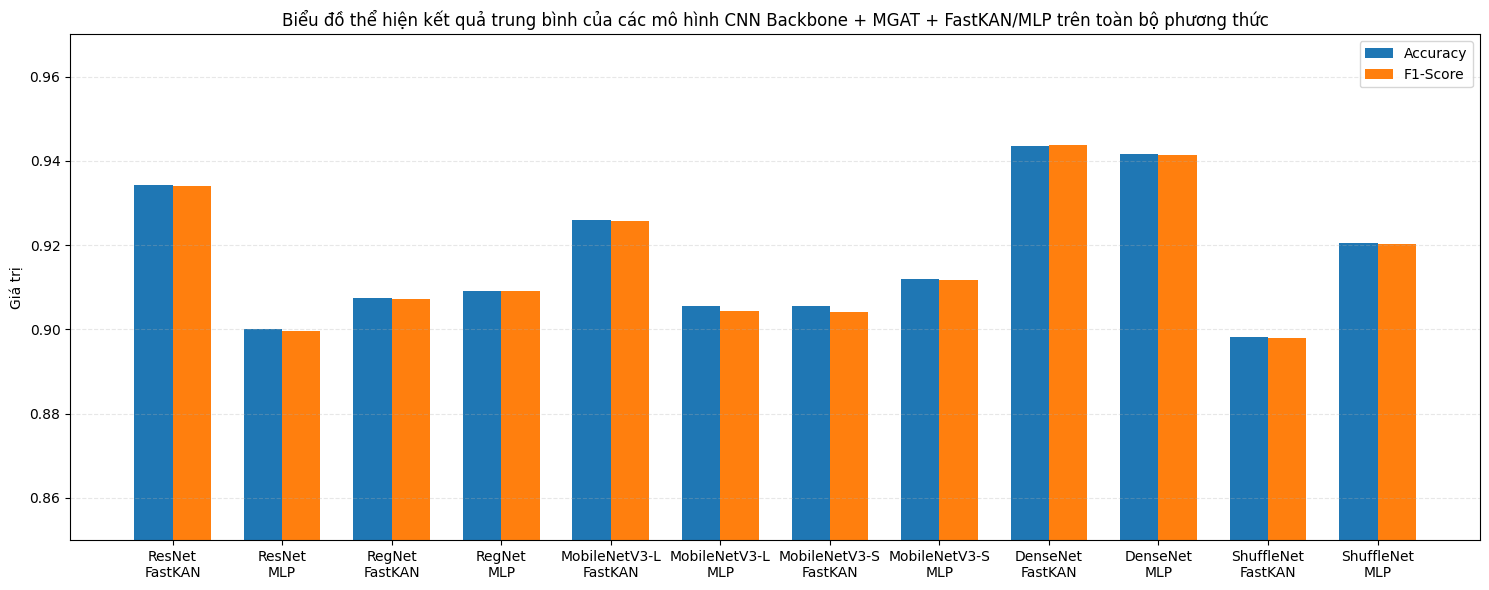
\includegraphics[width=\linewidth]{images/part-02/chap-03/sec-02/PipelineFull.png}
    \caption{\centering Biểu đồ thể hiện kết quả kiểm thử trung bình của tất cả các mô hình CNN backbone + MGAT + FastKAN/MLP trên toàn bộ phương thức}
    \label{fig:KQPipelineFull}
\end{figure}

% \indent Dựa trên bảng tổng hợp và biểu đồ thể hiện kết quả trung bình của 12 mô hình trên toàn bộ phương thức, tôi đưa ra các kết luận sau:\vspace{-0.1cm}
% \begin{itemize}[label={--}, itemsep=1pt]
%     \item \textbf{Khẳng định tính hiệu quả của phương pháp đề xuất:} Hầu hết các mô hình MGAT (dù kết hợp với FastKAN hay MLP) đều vượt qua ngưỡng hiệu năng của CNN Baseline (cao nhất ~0.90). Nổi bật nhất là sự kết hợp DenseNet121 + MGAT + FastKAN đạt tới \textbf{0.9435} và ResNet18 + MGAT + FastKAN đạt \textbf{0.9343}. Điều này chứng minh rằng việc mô hình hóa dữ liệu dưới dạng đồ thị đa phương thức đã thành công trong việc tận dụng thông tin bổ trợ từ văn bản và âm thanh để bù đắp các khoảng trống tri thức mà mô hình đơn phương thức bỏ sót.
%     \item \textbf{Sự tương quan giữa FastKAN và MLP:} Kết quả kiểm thử chỉ ra không có một bộ phân lớp nào là tối ưu cho mọi trường hợp:
%     \begin{itemize}[label={+}, itemsep=1pt]
%         \item \textbf{FastKAN} là lựa chọn tối ưu cho các mô hình có khả năng trích xuất đặc trưng mạnh (backbone lớn/sâu như ResNet, DenseNet, MobileNet Large). Khả năng biểu diễn hàm linh hoạt của KAN giúp khai thác triệt để lượng thông tin phong phú từ các backbone, điều này đã giúp đẩy độ chính xác phân lớp lên mức cao hơn.
%         \item \textbf{MLP} lại là giải pháp an toàn và hiệu quả cho các mô hình gọn nhẹ (backbone nhỏ như MobileNet Small, ShuffleNet). Trong trường hợp tài nguyên tính toán cực kỳ hạn chế, sự kết hợp ShuffleNetV2 + MLP (0.9204) mang lại kết quả rất ấn tượng.
%     \end{itemize}
% \end{itemize}

\indent Dựa trên bảng tổng hợp và các biểu đồ thể hiện kết quả trung bình của 12 mô hình trên toàn bộ phương thức, có thể rút ra những kết luận chính sau:\vspace{-0.1cm}
\begin{itemize}[label={--}, itemsep=1pt]
    \item Khẳng định hiệu quả của phương pháp đề xuất: Phần lớn các mô hình sử dụng MGAT (kết hợp với FastKAN hoặc MLP) cho ra kết quả cao hơn so với mô hình CNN baseline (cao nhất khoảng 0.91). Nổi bật nhất trong số đó là sự kết hợp của mô hình DenseNet121 + MGAT + FastKAN với độ chính xác đạt \textbf{0.9435} và ResNet18 + MGAT + FastKAN đạt 0.9343. Kết quả này cho thấy việc mô hình hóa dữ liệu dưới dạng đồ thị đa phương thức là một phương pháp xử lý hiệu quả các thông tin bổ trợ từ văn bản và âm thanh, qua đó bù đắp những hạn chế của các mô hình đơn phương thức.
    \item Mối quan hệ giữa FastKAN và MLP: Kết quả kiểm thử cho thấy không tồn tại một bộ phân lớp duy nhất có thể tối ưu cho mọi kiến trúc backbone:
    \begin{itemize}[label={+}, itemsep=1pt]
        \item FastKAN phù hợp hơn với các backbone có năng lực trích xuất đặc trưng mạnh (các kiến trúc lớn hoặc sâu như ResNet, DenseNet và MobileNetV3 Large). Nhờ khả năng biểu diễn hàm linh hoạt, FastKAN có thể khai thác hiệu quả lượng thông tin giàu ngữ nghĩa từ các đặc trưng đầu vào, qua đó giúp cải thiện đáng kể độ chính xác phân lớp.
        \item MLP cho ra kết quả ổn định hơn đối với các backbone gọn nhẹ (như MobileNetV3 Small và ShuffleNet). Trong bối cảnh tài nguyên tính toán bị giới hạn nghiêm ngặt, sự kết hợp ShuffleNetV2 + MLP (Accuracy đạt 0.9204) vẫn mang lại kết quả rất ấn tượng..
    \end{itemize}
\end{itemize}